\documentclass[tikz,border=12pt]{standalone}
\usepackage{tikz}
\usetikzlibrary{arrows.meta}

\definecolor{fairblue}{RGB}{33, 102, 172}
\definecolor{fairmidblue}{RGB}{103, 169, 207}
\definecolor{fairlight}{RGB}{247, 247, 247}
\definecolor{fairmidred}{RGB}{239, 138, 98}
\definecolor{fairred}{RGB}{178, 24, 43}
\definecolor{darkgray}{RGB}{50, 50, 50}
\definecolor{lightgrid}{RGB}{230, 230, 230}

\begin{document}
\begin{tikzpicture}[font=\sffamily, >=Stealth]
  % Panel a: Multi-Compartment Cellular Cross-Section
  \node[font=\large\bfseries] at (0, 14.2) {a};
  \node[anchor=west, font=\small\bfseries, text=darkgray] at (0.4, 14.2) {Mycobacterium marinum Multi-Compartment Cellular and Metabolic Architecture};

  % Layer 1: Substrate & Outer Mycomembrane (Capsule)
  \draw[line width=2pt, draw=gray!40] (0.2, 13.5) -- (13.5, 13.5);
  \node[anchor=west, font=\tiny\bfseries, text=gray!80!black] at (0.2, 13.7) {PDMS Silicone Membrane Substrate (Quiescent Boundary Layer)};

  % Outer Mycomembrane Strip
  \fill[fairmidred!20] (0.2, 12.3) rectangle (13.5, 13.1);
  \draw[thick, draw=fairmidred] (0.2, 13.1) -- (13.5, 13.1);
  \draw[thick, draw=fairmidred] (0.2, 12.3) -- (13.5, 12.3);
  \node[anchor=west, font=\tiny\bfseries, text=fairred!80!black] at (0.3, 12.7) {Outer Mycomembrane: Cord Factor (TDM) \& GPL Biofilm Matrix};

  % Extracellular/Capsular elements
  \node[fill=fairblue, text=white, font=\tiny\bfseries, rounded corners=2pt, inner sep=2pt] at (3.2, 12.7) {mps1/2};
  \node[fill=fairred, text=white, font=\tiny\bfseries, rounded corners=2pt, inner sep=2pt] at (6.5, 12.7) {fbpA (+1.2)};
  \node[anchor=west, font=\tiny, text=darkgray] at (7.4, 12.7) {Cord Factor (TDM) Deposition};
  \node[fill=fairblue, text=white, font=\tiny\bfseries, rounded corners=2pt, inner sep=2pt] at (11.5, 12.7) {espB (-6.0)};

  % Layer 2: Periplasmic Space & Arabinogalactan-Peptidoglycan (AG-PG) Mesh
  \fill[gray!6] (0.2, 10.9) rectangle (13.5, 12.3);
  \draw[dashed, draw=gray!40] (0.2, 11.6) -- (13.5, 11.6);
  \node[anchor=west, font=\tiny\bfseries, text=darkgray] at (0.3, 11.95) {Periplasmic Space: Arabinogalactan-Peptidoglycan Polymer Mesh};
  
  \node[fill=fairmidred, text=white, font=\tiny\bfseries, rounded corners=2pt, inner sep=2pt] at (2.2, 11.3) {murA (+0.8)};
  \node[anchor=west, font=\tiny] at (3.0, 11.3) {Murein cross-linking};
  \node[fill=fairred, text=white, font=\tiny\bfseries, rounded corners=2pt, inner sep=2pt] at (7.8, 11.3) {mmpL3 (+1.1)};
  \node[anchor=west, font=\tiny] at (8.7, 11.3) {TMM Translocase};

  % Layer 3: Inner Plasma Membrane
  \fill[fairblue!15] (0.2, 9.1) rectangle (13.5, 10.9);
  \draw[thick, draw=fairblue] (0.2, 10.9) -- (13.5, 10.9);
  \draw[thick, draw=fairblue] (0.2, 9.1) -- (13.5, 9.1);
  \node[anchor=west, font=\tiny\bfseries, text=fairblue!90!black] at (0.3, 10.6) {Inner Plasma Membrane: Embedded Respiratory Complexes \& Translocons};

  % Membrane Complexes (Nodes)
  % Complex I (nuoC, nuoD)
  \draw[fill=fairred, draw=fairred!80!black, rounded corners=2pt] (0.4, 9.3) rectangle (1.9, 10.3);
  \node[font=\tiny\bfseries, text=white, align=center] at (1.15, 9.8) {Complex I\\nuoC/D (+6.6)};
  \draw[->, thick, draw=fairred] (1.15, 9.2) -- (1.15, 10.4) node[above, font=\tiny\bfseries] {4H$^+$};

  % Menaquinone reductase MenJ
  \draw[fill=fairred, draw=fairred!80!black, rounded corners=2pt] (2.3, 9.3) rectangle (3.5, 10.3);
  \node[font=\tiny\bfseries, text=white, align=center] at (2.9, 9.8) {MenJ\\(+6.2)};

  % Microaerophilic Cytochrome bd Oxidase (cydA, cydB)
  \draw[fill=fairred, draw=fairred!80!black, rounded corners=2pt] (3.9, 9.3) rectangle (5.4, 10.3);
  \node[font=\tiny\bfseries, text=white, align=center] at (4.65, 9.8) {Cyt $bd$\\cydA (+2.4)};
  \draw[->, thick, draw=fairred] (4.65, 9.2) -- (4.65, 10.4) node[above, font=\tiny] {O$_2 \to$ H$_2$O};

  % CydD Thiol ABC Exporter
  \draw[fill=fairred, draw=fairred!80!black, rounded corners=2pt] (5.8, 9.3) rectangle (7.0, 10.3);
  \node[font=\tiny\bfseries, text=white, align=center] at (6.4, 9.8) {CydD\\(+6.2)};
  \draw[->, thick, draw=fairred] (6.4, 9.2) -- (6.4, 10.4) node[above, font=\tiny] {Thiol};

  % Type VII ESX-1 Core Pore (eccB1, eccD1, eccE1)
  \draw[fill=fairmidred, draw=fairmidred!80!black, rounded corners=2pt] (7.4, 9.3) rectangle (9.0, 10.3);
  \node[font=\tiny\bfseries, text=white, align=center] at (8.2, 9.8) {Type VII\\eccB/D/E};
  \draw[->, thick, draw=fairmidred] (8.2, 9.2) -- (8.2, 12.3) node[midway, right=1pt, font=\tiny] {EsxA};

  % ATP Synthase
  \draw[fill=white, draw=gray!60, rounded corners=2pt] (9.4, 9.3) rectangle (10.6, 10.3);
  \node[font=\tiny\bfseries, text=darkgray, align=center] at (10.0, 9.8) {ATP Synth\\atpA (0.0)};
  \draw[<-, thick, draw=gray!60] (10.0, 9.2) -- (10.0, 10.4) node[below, font=\tiny] {ATP};

  % Alternate Transporters
  \draw[fill=fairblue, draw=fairblue!80!black, rounded corners=2pt] (11.0, 9.3) rectangle (12.2, 10.3);
  \node[font=\tiny\bfseries, text=white, align=center] at (11.6, 9.8) {fadD7\\(-5.3)};

  % Layer 4: Cytoplasm (Metabolic Cascades)
  \fill[fairlight] (0.2, 5.0) rectangle (13.5, 9.1);
  \node[anchor=west, font=\tiny\bfseries, text=darkgray] at (0.3, 8.8) {Cytoplasm: Biochemical Cascades \& Metabolic Shunts};

  % Cascade A: Nitrogen & Polyamine Shunt
  \draw[thick, draw=fairred!40, fill=white] (0.4, 5.2) rectangle (4.3, 8.5);
  \node[font=\tiny\bfseries, text=fairred, anchor=west] at (0.5, 8.2) {1. Nitrogen \& Polyamine Shunt};
  \node[font=\tiny, anchor=west] at (0.5, 7.7) {Carbamoyl-P + L-Ornithine};
  \draw[->, thick, draw=fairred] (1.8, 7.5) -- (1.8, 6.7);
  \node[fill=fairred, text=white, font=\tiny\bfseries, rounded corners=2pt, inner sep=2pt] at (1.8, 7.1) {argF (+7.0)};
  \node[font=\tiny, anchor=west] at (0.5, 6.4) {$\longrightarrow$ L-Citrulline $\to$ Polyamines};
  \node[fill=fairred, text=white, font=\tiny\bfseries, rounded corners=2pt, inner sep=2pt] at (2.2, 5.8) {ilvB / als (+6.1)};
  \node[font=\tiny, anchor=west] at (0.5, 5.4) {Pyruvate $\to$ 2-Acetolactate};

  % Cascade B: FAS-II Mycolic Acid Synthesis
  \draw[thick, draw=fairmidred!40, fill=white] (4.6, 5.2) rectangle (8.6, 8.5);
  \node[font=\tiny\bfseries, text=fairred!90!black, anchor=west] at (4.7, 8.2) {2. Mycolic Acid FAS-II Spiral};
  \node[font=\tiny, anchor=west] at (4.7, 7.7) {Acetyl-CoA $\xrightarrow{\textbf{accD}}$ Malonyl-CoA};
  \draw[->, thick, draw=fairmidred] (6.4, 7.5) -- (6.4, 6.7);
  \node[fill=fairred, text=white, font=\tiny\bfseries, rounded corners=2pt, inner sep=2pt] at (6.4, 7.1) {kasA (+1.8)};
  \node[font=\tiny, anchor=west] at (4.7, 6.4) {$\beta$-ketoacyl-AcpM $\xrightarrow{\textbf{inhA}}$ Acyl-AcpM};
  \node[font=\tiny, anchor=west] at (4.7, 5.8) {Meromycolate C70--C90 synthesis};
  \node[font=\tiny\bfseries, text=fairred!80!black, anchor=west] at (4.7, 5.4) {Cell Envelope Fortification};

  % Cascade C: Central Carbon & Redox Systems
  \draw[thick, draw=fairblue!40, fill=white] (8.9, 5.2) rectangle (13.3, 8.5);
  \node[font=\tiny\bfseries, text=fairblue!90!black, anchor=west] at (9.0, 8.2) {3. Redox \& Cofactor Systems};
  \node[fill=fairred, text=white, font=\tiny\bfseries, rounded corners=2pt, inner sep=2pt] at (10.0, 7.7) {adhP (+7.0)};
  \node[font=\tiny, anchor=west] at (10.7, 7.7) {Alcohol redox};
  \node[fill=fairred, text=white, font=\tiny\bfseries, rounded corners=2pt, inner sep=2pt] at (10.0, 7.0) {ribD (+6.2)};
  \node[font=\tiny, anchor=west] at (10.7, 7.0) {Riboflavin / FAD};
  \node[fill=fairred, text=white, font=\tiny\bfseries, rounded corners=2pt, inner sep=2pt] at (10.0, 6.3) {F420 (+6.0)};
  \node[font=\tiny, anchor=west] at (10.7, 6.3) {LLM oxidoreductase};
  \node[fill=fairblue, text=white, font=\tiny\bfseries, rounded corners=2pt, inner sep=2pt] at (10.0, 5.6) {icl1 (-0.7)};
  \node[font=\tiny, anchor=west] at (10.7, 5.6) {Glyoxylate bypass};

  % Panel b: Subsystem Perturbation Index (SPI) Bar Plot with Zero Overlap
  \node[font=\large\bfseries] at (0, 4.4) {b};
  \node[anchor=west, font=\small\bfseries, text=darkgray] at (0.4, 4.4) {Empirical Subsystem Perturbation Index (SPI) Ranking};

  % Axes raised with generous clearance for X-axis title
  \draw[->, thick] (4.8, 1.0) -- (12.6, 1.0) node[midway, below=18pt, font=\scriptsize\bfseries] {Subsystem Perturbation Index (SPI)};
  \draw[thick] (4.8, 1.0) -- (4.8, 4.2);

  \foreach \x/\lbl in {4.8/0, 6.3/5, 7.8/10, 9.3/15, 10.8/20, 12.3/25} {
    \draw (\x, 0.9) -- (\x, 1.0) node[below=3pt, font=\tiny] {\lbl};
    \draw[dashed, draw=gray!20] (\x, 1.0) -- (\x, 4.2);
  }

  % Bars (Y positions: 3.8, 3.4, 3.0, 2.6, 2.2, 1.8, 1.4)
  % 1. Nitrogen Shunts & Polyamines (SPI = 24.52)
  \node[anchor=east, font=\scriptsize\bfseries] at (4.6, 3.8) {Nitrogen Shunts \& Polyamines};
  \fill[fairred] (4.8, 3.6) rectangle (12.16, 4.0);
  \node[anchor=west, font=\tiny\bfseries, text=fairred] at (12.25, 3.8) {24.5 (Active, $+6.6$)};

  % 2. Redox Homeostasis & Cofactors (SPI = 10.62)
  \node[anchor=east, font=\scriptsize\bfseries] at (4.6, 3.4) {Redox Homeostasis \& Cofactors};
  \fill[fairred!90!white] (4.8, 3.2) rectangle (7.99, 3.6);
  \node[anchor=west, font=\tiny\bfseries, text=fairred!90!black] at (8.09, 3.4) {10.6 (Active, $+3.5$)};

  % 3. Cellular Respiration & Energy (SPI = 5.27)
  \node[anchor=east, font=\scriptsize\bfseries] at (4.6, 3.0) {Cellular Respiration \& Energy};
  \fill[fairmidred] (4.8, 2.8) rectangle (6.38, 3.2);
  \node[anchor=west, font=\tiny\bfseries, text=fairmidred] at (6.48, 3.0) {5.3 (Active, $+2.5$)};

  % 4. Type VII Secretion & Virulence (SPI = 2.87)
  \node[anchor=east, font=\scriptsize\bfseries] at (4.6, 2.6) {Type VII Secretion \& Virulence};
  \fill[fairblue!70!white] (4.8, 2.4) rectangle (5.66, 2.8);
  \node[anchor=west, font=\tiny\bfseries, text=fairblue] at (5.76, 2.6) {2.9 (Repressed, $-0.5$)};

  % 5. GPL Biofilm & Cell Surface (SPI = 2.69)
  \node[anchor=east, font=\scriptsize\bfseries] at (4.6, 2.2) {GPL Biofilm \& Cell Surface};
  \fill[fairblue!60!white] (4.8, 2.0) rectangle (5.61, 2.4);
  \node[anchor=west, font=\tiny\bfseries, text=fairblue] at (5.71, 2.2) {2.7 (Repressed, $-0.9$)};

  % 6. Mycolic Acid & FAS-II Envelope (SPI = 1.24)
  \node[anchor=east, font=\scriptsize\bfseries] at (4.6, 1.8) {Mycolic Acid \& FAS-II Envelope};
  \fill[fairmidred!60!white] (4.8, 1.6) rectangle (5.17, 2.0);
  \node[anchor=west, font=\tiny\bfseries, text=fairmidred!80!black] at (5.27, 1.8) {1.2 (Active, $+0.4$)};

  % 7. DosR Hypoxia & Central Carbon (SPI = 0.97)
  \node[anchor=east, font=\scriptsize\bfseries] at (4.6, 1.4) {DosR Hypoxia \& Central Carbon};
  \fill[fairblue!40!white] (4.8, 1.2) rectangle (5.09, 1.6);
  \node[anchor=west, font=\tiny\bfseries, text=gray!80!black] at (5.19, 1.4) {0.97 (Baseline shift)};
\end{tikzpicture}
\end{document}
